\documentclass{beamer}
%[handout] option gets rid of extra frames
%\hypersetup{colorlinks=true,
%linkcolor=blue,
%citecolor=red,
%urlcolor=red,
%}
%\usetheme{Darmstadt}
%\usetheme{default}
\usetheme{Boadilla}
 %\usetheme{Madrid}
% \usetheme{Montpellier}
% \usetheme{Warsaw}
% \usetheme{Copenhagen}
% \usetheme{Goettingen}
% \usetheme{Hannover}
%\usetheme{Berkeley}
\numberwithin{equation}{section}
\setbeamertemplate{footline}[page number]{}
\usepackage{lmodern}
\usepackage{tikz}
\synctex=1
\setbeamercovered{transparent}
%\setlength{\parindent}{0in} %no indentation of paragraphs after section title
%
\newcommand{\rr}{\mathbb{R}}
\newcommand{\p}{\partial}
\newcommand{\zz}{\mathbb{Z}}
\newcommand{\cc}{\mathbb{C}}
\newcommand{\ci}{\mathbb{T}}
\newcommand{\tor}{\mathbb{T}}
\newcommand{\ee}{\varepsilon}
\newcommand{\wh}{\widehat}
\newcommand{\weak}{\rightharpoonup}
\newcommand{\vp}{\varphi}
%
%
\newtheorem{proposition}{Proposition}
\newtheorem{claim}{Claim}
\newtheorem{remark}{Remark}
\newtheorem{conjecture}[subsection]{conjecture}

%%%%%%%%%%%%%%%%%%%%%%
%
\date{}
\title{An Introduction to the Hyperelastic Rod Equation}
\author{David Karapetyan}
\institute{University of Rochester}
\begin{document}

\begin{frame}
    \titlepage
\end{frame}


\section*{Table of Contents}
\setcounter{section}{0}
\begin{frame}
	\frametitle{Table Of Contents}
	    \tableofcontents
	\end{frame}
	\section{Introduction}
        \begin{frame}
            \frametitle{Introduction}
We consider the hyperelastic rod (HR) Cauchy problem written in non-local form
\begin{gather*}
 \p_t u =  -\gamma u \p_x u -
 \p_{x} (1 - \p_{x}^{2})^{-1} \left[ \frac{3-\gamma}{2}u^2 +
\frac{\gamma}{2} \left( \p_x u \right)^2
\right], \ \gamma \neq 0,
\label{hyperelastic-rod-equation}
\\
 u(x,0) = u_0(x), \; \; x \in \rr, \; \; t \in \rr
\label{init-cond}
\end{gather*}
\begin{itemize}
        \pause
    \item
        Derived by Dai as a one-dimensional 
        model for finite-length and
        small-amplitude axial deformation waves in thin cylindrical
        rods composed of a compressible Mooney-Rivlin
        material. The derivation relied upon a reductive perturbation technique.
    \item 
       \pause 
       Well-posedness in $H^{s}$, $s > 3/2$ shown by Yin [2003]
       and Zhou [2005]
        for line and circle.
    \item 
       \pause 
        Alternative proof of well-posedness using a Galerkin method
	outlined by Taylor [1993], and shown by Karapetyan [2010]. 
   \pause 
\item 
    Special Feature: Unlike KDV, admits peakon ($\gamma > 0$) and cusped
    solutions ($\gamma \neq 0$).
\end{itemize}
\end{frame}

\subsection{CH Theory}
\begin{frame}
  \frametitle{CH Theory}
  \begin{itemize}
    \item
CH ($\gamma =1$) admits solutions of form
%
\begin{equation*}
  u(x,t)= p e^{-| x + q |} - p e^{-| x-q |},
\end{equation*}
%
where $p=p(t)$ and  $q=q(t)$ are positive functions of $t$
satisfying
%
\pause
\begin{align*}
  &p' = p^2 e^{-2q}, \\
  &q' = p (e^{-2q} -1).
\end{align*}
\end{itemize}
\pause
Crucial in proving following:
\end{frame}
\begin{frame}
  \begin{lemma}
  %
  %
  For $r < s < 3/2$,
  %
  %
  \begin{equation*}
    \begin{split}
      \lim_{t \to T^{-}}
      \frac{\|u(t)\|_{H^{r}(\rr)}}{\|u(t)\|_{H^{s}(\rr)}} = 0.
    \end{split}
  \end{equation*}
  \end{lemma}
  \pause
  and
  \begin{lemma}
  Let $ \ee >0$ and $ 1/2< s < 3/2$. If $q \le c_s \ee$, then 
  %
  %
  \begin{equation*}
    \label{peakon-antipeakon-Hs-bound}
    \begin{split}
      \|e^{-| x+ q |} - e^{-| x- q |} \|_{H^{s}(\rr)} < \ee^{3/2 - s}.
    \end{split}
  \end{equation*}
  Here $c_s$ is a constant depending only on $s$. 
  %
\end{lemma}
  %
\pause
Taken together, obtain failure of continuity for the data-to-solution map.

\end{frame}
\subsection{BBM Theory}
\begin{frame}
  \frametitle{BBM Theory}
  \begin{itemize}
    \item 
      For BBM ($\gamma = 0$) have an entirely different theory---it is a \emph{dispersive} equation
      \pause
     \begin{gather*}
 \p_t u = - 
 \frac{3}{2}\p_{x} (1 - \p_{x}^{2})^{-1} u^{2}, \ \gamma \neq 0,
\\
 u(x,0) = u_0(x), \; \; x \in \rr, \; \; t \in \rr
\end{gather*}
\pause
\item More precisely, Bona and Tzvetkov [2009] proved the following bilinear estimate:
  \begin{lemma}
    For $s \ge 0$, 
    \[ \| \p_{x}(1 - \p_{x}^{2})^{-1} (uv)\|_{H^{s}} \lesssim \| u \|_{H^{s}} \| v \|_{H^{s}}. \]
  \end{lemma}
  \pause
\item In fact, they showed that this bilinear estimate is sharp. Failure of continuity for $s < 0$ using a technique pioneered by Bejenaru and Tao [2006] was shown by Panthee [2010]. For a clear exposition of the technique, see Geba, Himonas, and Karapetyan [2012].
\end{itemize}
\end{frame}
\subsection{HR, $\gamma \neq 0,1$ Theory}
\begin{frame}
  \frametitle{HR, $\gamma \neq 0,1$ Theory}
  For $\gamma \neq 1$, don't have peakon anti-peakon interaction. For $\gamma \neq 0,1$, best ill-posedness result currently known is the following.
  \pause
\begin{theorem}
Let $\gamma$ be a nonzero constant. Then 
the data-to-solution map $u(0) \mapsto u(t)$ of the Cauchy-problem
for the HR equation
is not uniformly continuous
from any bounded subset of  $H^s$ into $C([-T, T], H^s)$
for $s>3/2$ on the line and circle.
%
\end{theorem}
\pause
\begin{itemize}
  \item
    Uses method of approximate solutions, motivated by work of Himonas-Kenig [2009], Himonas-Kenig-Misiolek [2010]. 
  \item 
See also Burq-G{\'e}rard-Tzvetkov [2002].
\end{itemize}
\end{frame}
\section{New Results on H\"older Continuity for HR}
\begin{frame}
  \frametitle{New Results}
  \begin{itemize}
      \pause
    \item
  Notion of continuity, and even uniform continuity, while mathematically interesting, are not numerically all that interesting. 
  \pause
\item
  Lipschitz continuity, or H\"older continuity, on the other hand, gives us an excellent quantitative understanding of how the size of the difference of two solutions changes as the size of the difference of their corresponding initial data changes.
  \pause
\item
  Hence, motivated by Chen, Liu, and Zhang [2011] we show the
following result:
\end{itemize}
\end{frame}
\begin{frame}


\begin{theorem}
For $\gamma \neq 0$, the
data to solution map for HR is H\"older continuous from $B_{H^{s}}(R)$ (in
the topology of $H^{r}$) to $C([0, T], H^{r})$, where $T = T(R)$, for $s >
3/2$, $-1 \le r < s$. More
precisely, consider the following sets 

  
  \begin{equation*}
  \begin{split}
      & \Omega_{1} = \left\{ (s, \ r) \in \rr^{2}:
     \ s>3/2, \ -1 \le r \le s-1, \ s + r \ge 2  \right\}
    \\
    & \Omega_{2} = \left\{ (s, \ r) \in \rr^{2}:
     \ s>3/2, \ -1 \le r < 2-s \right\}
    \\
    & \Omega_{3} = \left\{ (s, \ r) \in \rr^{2}:
    \  s>3/2, \  s-1 < r < s  \right\}.
    \end{split}
\end{equation*}
\end{theorem}
\end{frame}
\begin{frame}
\begin{theorem}
\begin{center}
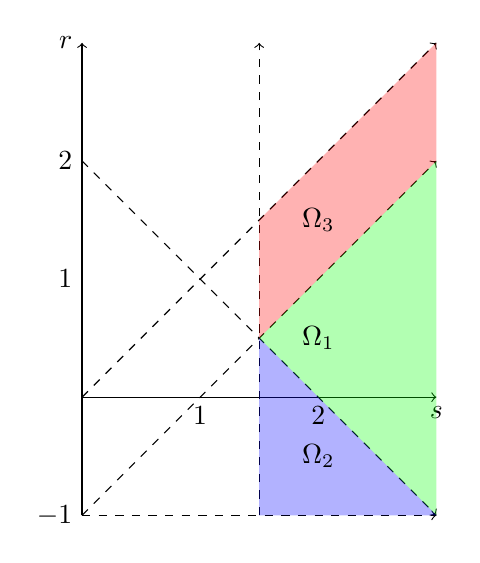
\begin{tikzpicture}[scale=1.5]
Draw thin grid lines with color 40% gray + 60% white

Draw x and y axis lines
\draw [->] (0,0) -- (3,0) node [below] {$s$};
\draw [->] (0,-1) -- (0,3) node [left] {$r$};
\draw [->, dashed] (0,0) -- (3,3);
\draw [->, dashed] (0,-1) -- (3,2);
\draw [->, dashed] (0,2) -- (3,-1);
\draw [->, dashed] (0,-1) -- (3,-1);
\draw [->, dashed] (3/2,-1) -- (3/2, 3);
\fill[color=green, fill opacity=0.3] (1.5, 0.5) -- (3,2) -- (3,0) -- (3,-1);
\fill[color=red, fill opacity=0.3] (1.5, 0.5) -- (1.5,1.5) -- (3,3) -- (3,2);
\fill[color=blue, fill opacity=0.3] (1.5, 0.5) -- (1.5, -1) -- (3, -1);


\foreach \x/\xtext in {1, 2}
    \draw[shift={(\x,0)}]  node[below] {$\xtext$};
\foreach \y/\ytext in {-1, 1, 2}
    \draw[shift={(0,\y)}]  node[left] {$\ytext$};
    \draw (2,1.5) node {$\Omega_{3}$};
    \draw (2,0.5) node {$\Omega_{1}$};
    \draw (2,-0.5) node {$\Omega_{2}$};
\end{tikzpicture}
\end{center}


Then for two initial data $u_{0}, v_{0} \in B_{H^{s}}(R)$, there exist unique
corresponding solutions $u(x,t), v(x,t)$ for $0 \le t \le T= T(R)$ to the
HR equation which satisfy 
\end{theorem}
\end{frame}
\begin{frame}
    \begin{theorem}

\begin{equation*}
\begin{split}
  \| u(t) - v(t) \|_{H^{r}} \le C \| u_{0} - v_{0} \|_{H^{r}}^{\alpha(s, r)},
  \quad 0
  \le t \le T
\end{split}
\end{equation*}


where 


\begin{equation*}
\begin{split}
\alpha = 
\begin{cases}
   1, \quad & (s,r) \in \Omega_{1} 
  \\
   2(s-1)/(s-r),  \quad & (s, r) \in \Omega_{2}
  \\
   s-r, \quad & (s, r) \in \Omega_{3}.
\end{cases}
\end{split}
\end{equation*}
\end{theorem}
\pause
\begin{itemize}
    \item
This result improves upon the H\"older continuity result in
Chen, Liu, and Zhang [2011] (there it is for $0 \le r < s$) by a full degree in $r$. 
\item Proof in periodic analogous to non-periodic
\end{itemize}

\end{frame}

\subsection{Region $\Omega_{1}$ $(-1 \le r \le s-1, \ s + r \ge 2$)} 
\begin{frame}


\frametitle{Region $\Omega_{1}$ $(-1 \le r \le s-1, \ s + r \ge 2$)} 

Let $u_{0}(x), v_{0}(x)
\in B_{H^{s}}(R)$, $s > 3/2$ be two initial datum. Then from
the well-posedness theory for HR  we
know that there exists unique corresponding solutions $u, v \in C(I,
B_{H^{s}}(2R))$ to the HR Cauchy problem.
Set $v=u-w$. Then $v$ solves the Cauchy-problem

\pause
\begin{align*}
& \p_t v
=  -\frac{\gamma}{2} \p_x [v(u + w)] 
\\
\notag
& \phantom{\p_t v = }-\p_x (1 - \p_{x}^{2})^{-1} \left\{
\frac{3-\gamma}{2}[v(u+w)] + \frac{\gamma}{2}[\p_x v \cdot \p_x (u+w)]
\right\},
\\
& v(x,0) = u_{0}(x) - v_{0}(x).
\end{align*}
\end{frame}

\begin{frame}
Let

\begin{equation*}
    D^{m} = (1 - \p_x^2)^{m/2}, \quad m \in \rr.
\end{equation*}

Applying $D^r$ to both sides then 
multiplying both sides by $D^r v$ and integrating, we obtain


\begin{equation*}
\begin{split}
 \frac{1}{2} \frac{d}{dt} \|v\|_{H^r}^2
 = & -\frac{\gamma}{2} \int_{\rr} D^r \p_x [v(u+w)] \cdot
D^r v \ dx
\\
& - \frac{3-\gamma}{2} \int_{\rr}  D^{r -2}
\p_x[v(u+w)] \cdot
D^r v \ dx  
\\
& - \frac{\gamma}{2} \int_{\rr} D^{r 
-2} \p_x [ \p_x v
\cdot \p_x (u+w)]\cdot D^r v \ dx.
\label{2v}
\end{split}
\end{equation*}
\end{frame}


\begin{frame}
\frametitle{Estimate of Integral 1} Note that


\begin{equation*}
\begin{split}
& \left |  -\frac{\gamma}{2} \int_{\rr} D^r \p_x [v(u+w)] \cdot
D^r v \ dx \right |
\\
& =
\left |
-\frac{\gamma}{2} \int_{\rr} \left[ D^r \p_x, \ u+w \right]v \cdot
D^r v \ dx - \frac{\gamma}{2} \int_{\rr} (u+w) D^r
\p_x v \cdot D^r v\ dx
\right | \\
& \lesssim \left |
\int_{\rr} \left[ D^r \p_x, \ u+w \right]v \cdot
D^r v \ dx \right |
+ \left | \int_{\rr} (u+w) D^r \p_x v
\cdot D^r v\
dx \right |.
\label{4v}
\end{split}
\end{equation*}

\pause

Observe that integrating by parts gives


\begin{equation*}
\begin{split}
\left | \int_{\rr} (u+w) D^r \p_x v \cdot
D^r v \ dx \right |
\le \|\p_x (u+w)\|_{L^\infty}
\|v\|_{H^r}^2.
\label{4'v}
\end{split}
\end{equation*}




\end{frame}

\begin{frame}
To estimate the remaining piece, we shall need the following
following result taken from Himonas [2010]:

    \begin{lemma}[Commutator Estimate]
\label{cor1}
If $s > 3/2$ and $-1 \le r  \le s -1$, then


\begin{equation*}
\begin{split}
\|[D^r \p_x ,f]g\|_{L^2} \le C \|f\|_{H^s} \|g\|_{H^r}.
\label{15}
\end{split}
\end{equation*}


\end{lemma}
\end{frame}

\begin{frame}
Set $s > 3/2$ and $-1 \le r \le s -1$. An application of 
Cauchy-Schwartz and the Commutator Estimate then yields 


\begin{equation*}
\begin{split}
 \left | \int_{\rr} [D^r \p_x, \ u+w] v
\cdot D^r v \ dx \right |
& \lesssim \|u+w\|_{H^s} 
\|v\|_{H^r}^2.
\label{7v}
\end{split}
\end{equation*}


\pause

Combining everything and applying the Sobolev Imbedding 
Theorem, we obtain 


\begin{equation*}
\begin{split}
\left |  -\frac{\gamma}{2} \int_{\rr} D^r \p_x [v(u+w)] \cdot
D^r v \ dx \right |
 \lesssim \|u+w\|_{H^s} \|v\|_{H^r}^2
\label{8v}
\end{split}
\end{equation*}
for $s > 3/2, \ -1 \le r \le s-1$.
\end{frame}

\begin{frame}
\frametitle{Estimate of Integral 2} 

%%%%%%%%%%%%%%%%%%%%%%%%%%%%%%%%%%%%%%%%%%%%%%%%%%%%%


               %frac deriv est


%%%%%%%%%%%%%%%%%%%%%%%%%%%%%%%%%%%%%%%%%%%%%%%%%%%%%


\begin{lemma}[Fractional Sobolev]
For $s > 3/2$, $r \le s$, $s + r \ge 2$, we have


\begin{equation*}
\begin{split}
  \| fg \|_{H^{r-1}} \lesssim \| f \|_{H^{r-1}} \| g \|_{H^{s-1}}.
\end{split}
\end{equation*}


\label{lem:frac-deriv}
\end{lemma}

%\begin{itemize}
    %\item  Improves upon estimate in Himonas and Kenig \cite{Himonas:2009fk}
        %\begin{equation*}
            %\| fg \|_{H^{\sigma -1}} \lesssim \| f \|_{H^{\sigma -1}} \| g
            %\|_{H^{\sigma}}, \quad 1/2 < \sigma < 1
        %\end{equation*}
%\end{itemize}

\end{frame}

\begin{frame}


Applying Cauchy-Schwartz and the Fractional Sobolev Lemma, we obtain



\begin{equation*}
\begin{split}
\left | - \frac{3-\gamma}{2} \int_{\rr}  D^{r -2}
\p_x[v(u+w)] \cdot
D^r v \ dx  \right |
 & \lesssim \|u+w\|_{H^{r -1}} \|v\|_{H^r}^2
\end{split}
\end{equation*}

\pause

which implies
\begin{equation*}
\begin{split}
\left | - \frac{3-\gamma}{2} \int_{\rr}  D^{r -2}
\p_x[v(u+w)] \cdot
D^r v \ dx  \right |
 & \lesssim \|u+w\|_{H^{s}} \|v\|_{H^r}^2
 \label{3v}
\end{split}
\end{equation*}

for $s > 3/2, \ r \le s, \ \text{and} \ s + r \ge 2$.

\end{frame}
\begin{frame}
\frametitle{Estimate of Integral 3} 

Applying Cauchy-Schwartz, the Fractional Sobolev Lemma and the inequality $\| f_{x}
\|_{H^{m-1}} \le \| f \|_{H^{m}}$,  we conclude that

\begin{equation*}
\begin{split}
\left | - \frac{\gamma}{2} \int_{\rr} D^{r 
-2} \p_x [ \p_x v
\cdot \p_x (u+w)]\cdot D^r v \ dx \right | 
 \lesssim \|u+w \|_{H^{s}}
\|v\|_{H^r}^2
\label{3'v}
\end{split}
\end{equation*}


for $s > 3/2, \ r \le s, \ \text{and} \ s + r \ge 2$.
\end{frame}
\begin{frame}
Grouping estimates for Integrals 1-3, get


\begin{equation*}
\begin{split}
\frac{1}{2} \frac{d}{dt}
\|v\|_{H^r}^2
& \lesssim \|u+w\|_{H^s}
\|v\|_{H^r}^2, \quad | t | < T
\\
& \le 4R \| v \|_{H^{r}}^{2}
\label{9v}
\end{split}
\end{equation*}

\pause
which by Gronwall gives

\begin{equation*}
  \label{lip-ineq}
\begin{split}
  & \| u(t) - w(t) \|_{H^{r}} \le C \| u_{0} - w_{0} \|_{H^{r}}, 
  \\
  & \text{for} \ | t | < T,
  \ s > 3/2, \ -1 \le r \le s-1, \ s + r \ge 2.
\end{split}
\end{equation*}

\pause

Hence, in region $\Omega_{1}$, the data to solution map is locally Lipschitz from
$B_{H^{s}(R)}$ (measured with the $H^{r}$
norm) to $C([-T, T], H^{r})$, with Lipschitz constant $C = C(s, r, R)$.

\end{frame}


\subsection{Region $\Omega_{2}$ $(-1 \le r < 2-s)$} 

\begin{frame}
\frametitle{Region $\Omega_{2}$ $(-1 \le r < 2-s)$} 

We have the estimate
\begin{equation*}
  \label{fgh}
\begin{split}
  \| v(t) \|_{H^{r}}
  & < \|v(t) \|_{H^{2-s}}.
    \end{split}
\end{equation*}

\end{frame}
\begin{frame}
We see that Lip inequality is valid for $r = 2-s$, $3/2 < s \le 3$.
Hence, applying it, we obtain 




\begin{equation*}
\begin{split}
\| v(t) \|_{H^{r}}
 \lesssim \|v(0) \|_{H^{2-s}}.
\end{split}
\end{equation*}





We need the following interpolation
result. 
 \end{frame} 

 \begin{frame}
     \begin{lemma}[Interpolation]
  For $m_{1} < m < m_{2}$,
  
  
  \begin{equation*}
  \begin{split}
    \| f \|_{H^{m}} \le \| f \|_{H^{m_{1}}}^{(m_{2}-m)/(m_{2} - m_{1})} \| f
    \|_{H^{m_{2}}}^{(m -m_{1})/(m_{2} - m_{1})}.
  \end{split}
  \end{equation*}
  
  
  
   
  
\label{lem:interp}
\end{lemma}

\pause
Applying the lemma with $m_{1} =r$, $m = 2-s$, and $m_{2} = s$ (notice
$m_{2} > m$ for $s > 1$), we bound 


\begin{equation*}
\begin{split}
    \| v(0) \|_{H^{2-s}} 
    & \le \| v(0) \|_{H^{r}}^{\frac{2(s-1)}{s-r}} \|v(0)
  \|_{H^{s}}^{\frac{2-s-r}{s-r}}
  \\
  & = \| u_{0} - w_{0} \|_{H^{r}}^{\frac{2(s-1)}{s-r}} \|u_{0} - w_{0}
  \|_{H^{s}}^{\frac{2-s-r}{s-r}}
  \\
  & \lesssim \| u_{0} - w_{0} \|_{H^{r}}^{\frac{2(s-1)}{s-r}}.
\end{split}
\end{equation*}

\pause
We conclude that


\begin{equation*}
\begin{split}
  \| u(t) - w(t) \|_{H^{r}} \lesssim \|u_{0} - w_{0} \|_{H^{r}}^{\frac{2(s-1)}{s-r}}.
\end{split}
\end{equation*}

\end{frame}

\subsection{Region $\Omega_{3}$ $(s-1 < r < s)$} 

\begin{frame}
\frametitle{Region $\Omega_{3}$ $(s-1 < r < s)$} 


Applying the Interpolation Lemma with $m_{1} = s-1$, $m =r$ and $m_{2} = s$ and
the estimate


\begin{equation*}
\begin{split}
  \|v\|_{H^{s}} = \|u - w \|_{H^{s}} \le 4R
\end{split}
\end{equation*}


we obtain


\begin{equation*}
  \label{pre-lip-ap}
\begin{split}
  \| v(t) \|_{H^{r}} & \lesssim \| v(t) \|_{H^{s-1}}^{s-r} \|v(t) \|_{H^{s}}^{1-s+r}
  \\
  & \simeq \| v(t) \|_{H^{s-1}}^{s-r}.
\end{split}
\end{equation*}


\end{frame}
\begin{frame}
We see that Lip inequality is valid for  $r = s-1$, $s \ge 3/2$. Hence,
applying it above we obtain 


\begin{equation*}
\begin{split}
    \|u(t) - w(t) \|_{H^{r}} = \| v(t) \|_{H^{r}} & \lesssim \|v(0) \|_{H^{s-1}}^{s-r}
   \\
   & \le \|v(0) \|_{H^{r}}^{s-r} 
  \\
  & = \|u_{0} - w_{0}\|_{H^{r}}^{s-r}.
\end{split}
\end{equation*}

\end{frame}
\section{Comments on Well-Posedness Proof for HR}
\begin{frame}
  \begin{center}
  \Large 
    Thank you
  \end{center}
\end{frame}
\end{document}
